\section{Curve-based island generation}
\label{sec:coral-island_example-generation}

% \begin{figure}
% 	\centering
% 	\autofitgraphics[]{placeholder.pdf}
%     \caption{The example generation fully takes its potential in the procedural techniques, using sketches from the user (top-view sketch, profile-view sketch, wind sketch, and resistance sketch) to generate a height field in accordance with a label map. }
%     \label{fig:coral-island_example-pipeline}
% \end{figure}

The generation of coral reef island terrains involves a structured process that takes the user's sketches and produces a complete 3D terrain model. This process begins with the creation of the initial height field based on the user's input, followed by the application of wind deformation to introduce natural variations, and concludes with the integration of coral reef features through subsidence and coral growth modeling.




The generation of coral reef islands in our system begins with two intuitive curve-based inputs from the user: a top-view sketch and a profile-view sketch, which define the islands horizontal layout and vertical elevation profile. In addition to these sketches, the user can further refine the terrain by applying wind deformation strokes, which simulate the effects of wind and waves on the islands shape. This combination of sketches and wind inputs gives users precise control over both the islands structure and its natural variations, such as irregular coastlines or concave features. We will present the usefulness of these sketches in this section, and describe the technical details in the next section.



\subsection{Initial height field generation}
\label{sec:coral-island_generation-initial}


% % \begin{figure}
% % 	\centering
% %     \autofitgraphics[]{Cicia_island.png, Cicia_island-outlines.png}
% % 	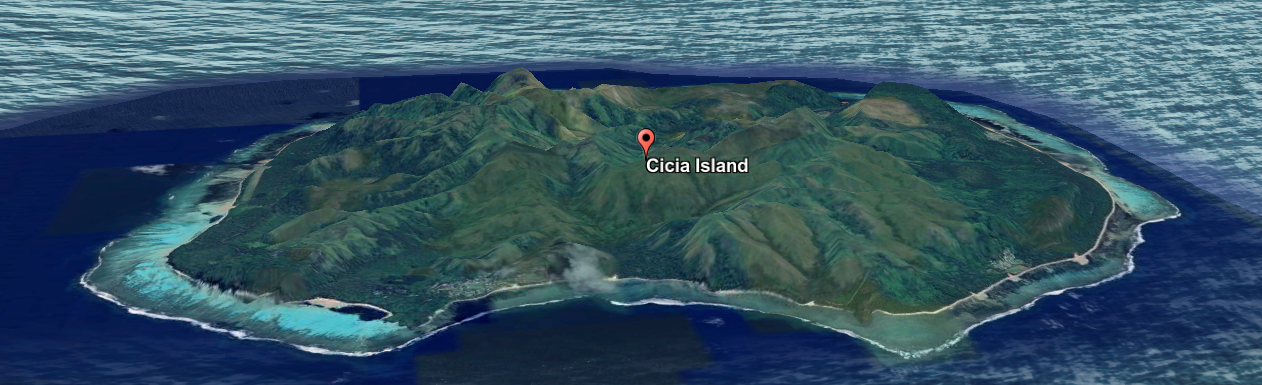
\includegraphics[width=0.90 \linewidth]{Cicia_island-3D.png}
% %     \caption{(Left) A real world example of aerial image (and 3D visualization on bottom) of an island (Cicia Island) may be segmented in regions. (Right) We can represent the different regions by the boundaries they form.}
% %     \label{fig:coral-island_top-view-sketch}
% % \end{figure}

% The top-view sketch defines the islands outline as seen from above. Using a simple drawing interface, the user can delineate the boundaries between key regions of the island, including the island itself, the beaches, the lagoon, and the surrounding abyss. The system assumes that these regions are arranged concentrically around the center of the island, with each boundary defined by a radial distance from the center.

% Each region's boundary is represented in polar coordinates, with $\radius_\p$ indicating the radial distance from the islands center and $\angl_\p$ representing the angular position. This polar representation allows the system to map the users sketch onto a circular framework, ensuring smooth transitions between regions and maintaining a coherent layout for the island.

% In this sketch, the user defines the overall horizontal layout of the island, including the size and shape of each feature. Variations in the outline are introduced by allowing the radial distances to vary with angle, ensuring that the island is not strictly symmetrical and introducing more natural, irregular shapes.

% \begin{figure}
%     \autofitgraphics[]{binary-heights-input-only-outlines-2.png, binary-heights-output-only-heightmap-2.png, binary-heights-render-2.png}
%     \caption{Using only the outlines of the island as a input sketch, we can provide a height to each point of the field depending on the region in which it rely.}
%     \label{fig:coral-island_procedural-height-only}
% \end{figure}



% % \begin{figure}
% % 	\centering
% %     \autofitgraphics[]{profileFunction.pdf, schema_profile.jpg}
% %     \caption{(Left) A profile function $\heightProfile$ is defined as a 1D function and represents the surface from the center of the island to the abysses. (Right) The cross-section representation of an island is often represented as a 1D function defined using terrain features as landmarks. }
% %     \label{fig:coral-island_profile-function}
% % \end{figure}

% The profile-view sketch defines the vertical elevation profile of the island along any radial direction, offering control over the islands height. In this view, the user specifies the elevation of different regions of the island, such as the island peak, beach, lagoon, abyss, and everything in-between, by drawing the corresponding profile curve.

% The regions outlines correspond to key terrain transitions: the highest point of the island (center), the island border, the beach, the lagoon, and the deep-sea abyss. The system uses these milestones to interpolate a continuous 1D height function $\heightProfile(\distRegions)$, where $\distRegions$ represents a non-uniform region distance from the islands center, and $h = \heightProfile(\distRegions)$ gives the height at each point. This continuous profile ensures smooth elevation transitions across the island.

% By combining the top-view and profile-view sketches, the system can generate a full 3D terrain model that accurately reflects the users design by revolution modeling.

% The generation of the coral reef island terrain begins by transforming the user-defined top-view and profile-view sketches into a coherent 3D height field. This process combines the radial layout of the top-view sketch with the elevation information provided by the profile-view sketch, creating a terrain that accurately represents the desired features, such as the island, beaches, lagoons, and abyss.

% For any point $\p$ on the terrain, the system first computes the polar coordinates $(\radius_\p, \angl_\p)$, where $\radius_\p$ is the radial distance from the island's center, and $\angl_\p$ is the angular component. The radial distance $\radius_\p$ is used to determine which region the point belongs to (island, beach, lagoon, reef, or abyss). The user-defined outlines in the profile sketch specify the radial limits between these regions.

% % \AltTextImage{
%     % Each point's height is determined by the profile function $\heightProfile(\distRegions)$, where $\distRegions$ represents a "piecewise parametric distance" from the island's center. The piecewise parametric distance works by dividing the radial distance from the center into segments, defined by these region boundaries. Each segment corresponds to a distinct region of the terrain, and within each segment, the distance $\distRegions$ is interpolated between the region boundaries. For a point $\p$ lying between two boundaries $\Radius_{i}$ and $\Radius_{i+1}$, the distance $\distRegions_\p$ is calculated as:

%     % \begin{align}
%     %     \distRegions_\p = i + \frac{\radius_\p - \Radius_{i}}{\Radius_{i + 1} - \Radius_{i}}
%     % \end{align}
%     % where $i$ is the index of the nearest lower region boundary. This method allows for smooth transitions between regions, even when the spacing between boundaries varies. 

%     % For any point $\p$, the height is finally computed as:
%     % \begin{align}
%     %     h(\p) = \heightProfile(\distRegions_\p)
%     % \end{align}
% % }{outlines-top-view-x-bar.pdf, outlines-result-x-bar.pdf}{The $\tilde{x}$ parameter is used to stretch the 1D height function $\heightProfile(x)$ to fit the distances from the center to the outlines of each region defined in the top-view sketch.}{fig:coral-island_parametric-distance}
% \wrapFig{outlines-top-view-x-bar.pdf}{.3}{label}{caption}

% Each point's height is determined by the profile function $\heightProfile(\distRegions)$, where $\distRegions$ represents a parametric region distance from the island's center. 

% Instead of using the raw radial distance $\radius_\p$, we define $\distRegions_\p$ to map each point to a normalized position along the sequence of terrain regions. The radial space is divided by the user-defined boundaries $\Radius_0, \Radius_1, ..., \Radius_n$ corresponding to the island, beach, lagoon, and abyss.

% For a point $\p$ lying between two boundaries $\Radius_{i}$ and $\Radius_{i+1}$, its parametric distance is defined as:

% \begin{align}
%     \distRegions_\p = i + \frac{\radius_\p - \Radius_{i}}{\Radius_{i + 1} - \Radius_{i}}
% \end{align}

% Here, $i$ is the index of the region containing $\p$ ($\Radius_i \leq \radius_\p < \Radius_{i+1}$). This formula maps the region's radial span to the interval $[i, i+1]$, ensuring smooth and consistent interpolation between adjacent regions.

% The final height at point $\p$ is computed by evaluating the elevation profile:
% \begin{align}
%     h(\p) = \heightProfile(\distRegions_\p)
% \end{align}
The top-view sketch defines the island's outline as seen from above. Using a simple drawing interface, the user delineates concentric boundaries for key regions such as the island itself, the beaches, the lagoon, and the surrounding abyss, around the canvas center. Each boundary is represented in polar coordinates, where $\radius_\p$ is the radial distance from the island's center and $\angl_\p$ is the angular position. Allowing $\radius$ to vary with $\angl$ introduces irregular, natural shapes rather than perfect circles (\cref{fig:coral-island_procedural-height-only}).

\begin{figure}
    \autofitgraphics[]{binary-heights-input-only-outlines-2.png, binary-heights-output-only-heightmap-2.png, binary-heights-render-2-corrected.png}
    % \autofitcaptions{User sketch , Height field , Rendered result }
    \caption{Using only the outlines from the top-view sketch, each point in the field is assigned a region (island, beach, lagoon, abyss), which later guides its height assignment.}
    \label{fig:coral-island_procedural-height-only}
\end{figure}

The profile-view sketch defines the island's vertical elevation along any radial direction. Here, the user draws a curve that specifies height at key terrain milestones, such as the central peak, island border, beach, lagoon, and abyss, creating a continuous 1D height function $\heightProfile(\distRegions)$ where $\distRegions$ is a parametric distance measuring position along the sequence of regions. This continuous profile ensures smooth elevation transitions across all terrain features.

\wrapFigR{outlines-x-bar.pdf}{.3}{fig:coral-island_parametric-distance}{Parametric distance $\tilde x$ depending on angle $\angl$. } %{The 3D terrain is generated by revolving the 1D height function $h(\tilde{x})$ around the center of the island. The colored base (green, yellow, blue) represents user-defined regions from the top-view sketch. The dark green surface corresponds to the elevation profile $h(\tilde{x})$, sampled along radial directions. Vertical slices show how each angle uses the same elevation curve.}

By combining the top-view and profile-view sketches via revolution modeling, the system generates a full 3D terrain model that matches the user's design. The process begins by transforming those two sketches into a coherent height field (\cref{fig:coral-island_procedural-smooth-heights}).

For any point $\p$ on the terrain, the system computes polar coordinates $(\radius_\p, \angl_\p)$. The radial distance $\radius_\p$ determines which region the point belongs to (island, beach, lagoon, reef, or abyss) based on the user-defined radial limits. Those outlines from the top-view sketch provide the exact boundaries between regions.

Each point's height is computed using the profile function $\heightProfile(\distRegions)$. Instead of using the raw radial distance $\radius_\p$, we define a parametric region distance $\distRegions_\p$ that maps each point to a normalized position along the concentric regions (see \cref{fig:coral-island_parametric-distance}). The radial space is divided by user-defined boundaries $\Radius_0, \Radius_1, \dots, \Radius_n$, corresponding to the island center, border, beach, lagoon, and abyss.

\begin{figure}[b]
    \autofitgraphics[]{smooth-input-outline-heights-1.png, smooth-output-heights-1.png, smooth-render-1-corrected.png}
    \autofitgraphics[]{smooth-input-outline-heights-2.png, smooth-output-heights-2.png, smooth-render-2-corrected.png}
    \autofitgraphics[]{smooth-input-outline-heights-3.png, smooth-output-heights-3.png, smooth-render-3-corrected.png}
    % \autofitcaptions{User outlines and profile, Height field, Rendered result}
    \caption{Providing a smooth function between each region results in islands with plausible reliefs. We fixed the outlines while editing only the height function in order to produce, from top to bottom, a low island, a coral reef island, and finally an identical island without the reef. }
    \label{fig:coral-island_procedural-smooth-heights}
    \label{fig:coral-island_procedural-smooth-heights-multiple-examples}
\end{figure}
When a point $\p$ lies between two boundaries, say $\Radius_{i}$ and $\Radius_{i+1}$, its parametric distance is
\begin{align}
    \distRegions_\p = i \;+\; \frac{\radius_\p - \Radius_{i}}{\Radius_{i + 1} - \Radius_{i}},
\end{align}
where $i$ is the index of the region containing $\p$ (i.e., $\Radius_i \le \radius_\p < \Radius_{i+1}$). This linear mapping stretches each region's radial span to the interval $[i,\,i+1]$, ensuring smooth interpolation across region boundaries. The final height at point $\p$ is then $h(\p) = \heightProfile(\distRegions_\p)$.
% \end{align}

% \begin{figure}
%     \autofitgraphics[]{smooth-input-outline-heights-1.png, smooth-output-heights-1.png, smooth-render-1.png}
%     \caption{Given top-view and side-view outlines, the 3D result is obtained by revolution. }
%     \label{fig:coral-island_procedural-smooth-heights}
% \end{figure}

% This approach ensures that the height field accurately follows the elevation profile specified by the user while maintaining smooth transitions between different regions of the island.

% The result is a height field that captures both the radial structure of the island (from the top-view sketch) and the vertical elevation profile (from the profile-view sketch), producing a realistic representation of islands with smooth transitions between the key terrain features.
\subsubsection{Wind deformation}
\label{sec:coral-island_wind-deformation}

% % \begin{figure}
% %     \centering
% %     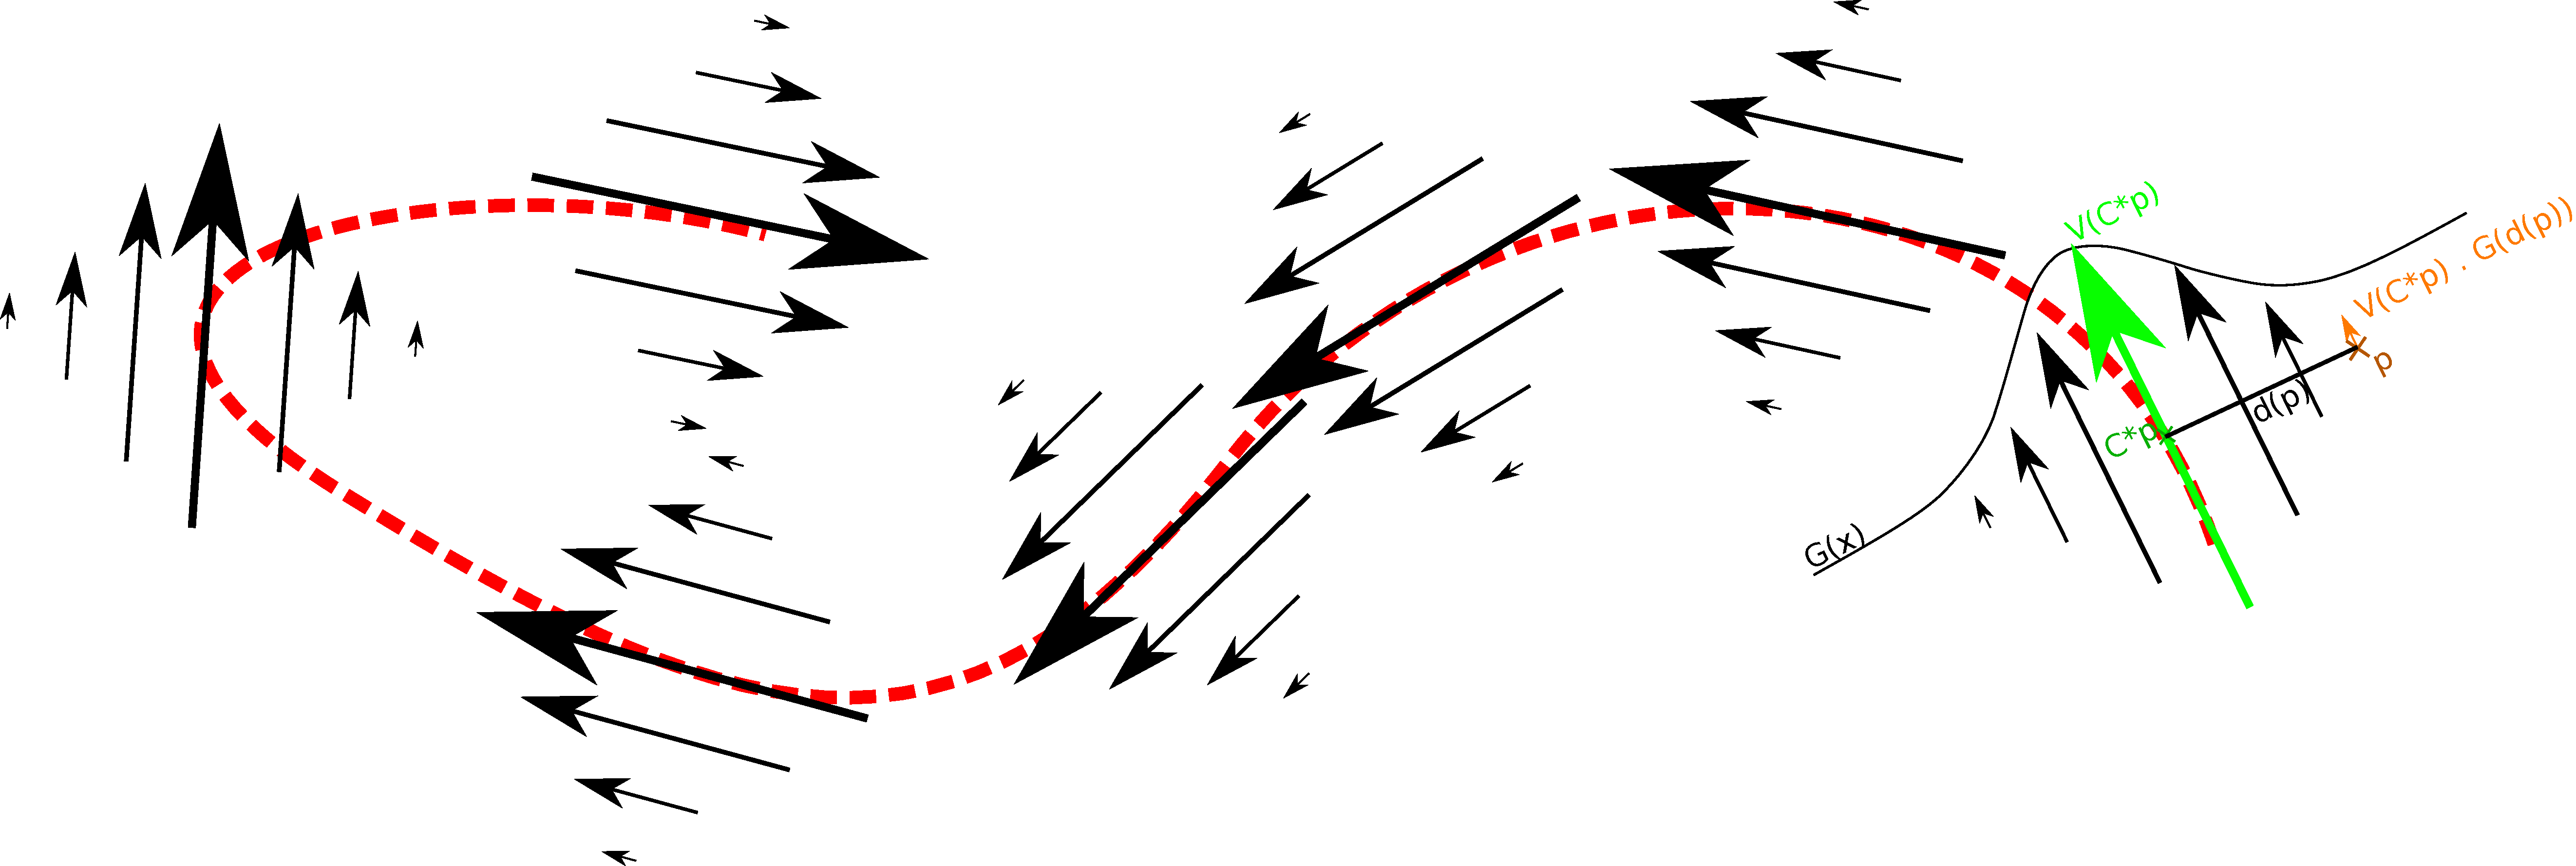
\includegraphics[width = 0.8 \linewidth]{windByStrokes.pdf}
% %     \caption{From the parametric curve defined by a user (red), we define the velocity field by considering the velocity (first derivative) of the curve at the closest point $\closestCp$, modulated by a gaussian distance function $G(x)$. }
% %     \label{fig:coral-island_wind-from-strokes}
% % \end{figure}

% In addition to the sketches, the user can influence the shape of the island by defining a wind velocity field. This field simulates the effects of wind and wave erosion on the island's surface, introducing natural deformations such as coastline indentations, and more importantly allow the user to break the radial symmetry constraint.

% The wind field is represented as a series of wind strokes drawn by the user on a 2D canvas. Each stroke represents a parametric curve, where the direction and strength of the wind are encoded as a vector field. The user controls the wind's direction by drawing these curves, and the system interprets the strokes to create a velocity field that defines how the terrain should be deformed.

% As the user draws a wind stroke, the system generates a set of control points along the curve, with the option to adjust the stroke's width. The width of each stroke determines the area of influence around the curve, where wider strokes result in broader deformations of the terrain.
% The deformation strength decreases with distance from the wind curve using a Gaussian falloff function using the stroke width as standard deviation, ensuring that the terrain transitions smoothly from deformed regions to non-deformed areas.
% Once the wind strokes are applied, the system processes the wind velocity field by displacing the terrain points accordingly. The height field, originally generated from the user's sketches, is modified by the wind field to create non-radial features, breaking the initial radial symmetry and producing a more organic island shape.

% After generating the initial height field based on the top-view and profile-view sketches, the next step in the process introduces wind deformation. This step simulates the long-term effects of wind and wave erosion, breaking the radial symmetry of the terrain and adding natural variations such as concave coastlines and irregular island shapes.

% The wind deformation can be controlled through a user-defined vector field, which represents the direction and strength of wind flows across the terrain. Users interact with the system by drawing strokes on a 2D canvas, which are then interpreted as parametric curves $\curve$ representing wind patterns. Each stroke defines a wind flow in the curve's direction $\curve'$, a strength $S$, and an effect width $\std$; these wind flows are used to displace the terrain, simulating the gradual reshaping of the island due to wind and wave erosion.

% The strokes are represented as Catmull-Rom splines, a type of parametric curve that allows for smooth, continuous wind paths. For any point $\p$ on the terrain, the deformation vector $\warp(\p)$ is calculated based on the proximity of $\p$ to the nearest wind strokes. The strength of the displacement is controlled by a Gaussian scaling function, which ensures that points closer to the wind strokes experience stronger displacement, while points farther away are less affected.

% The displacement function $\warp(\p)$ is computed as a sum of the influences from all nearby wind strokes. For each stroke, the deformation vector is scaled by a Gaussian function that smoothly decreases with the distance from $\closestCp$ the closest point on the parametric curve $\curve$, as follows:

% \begin{align}
%     \warp(\p) = \sum_{\curve \in \text{curves}} S \frac{\curve'(\q)}{\| \curve'(\q) \| } \cdot G_\std\left(\| \p - \closestCp \| \right)\\
%     G_\std(x) = \frac{1}{\std \sqrt{2\pi}} e^{-\frac{x^2}{2 \std^2}}
% \end{align}

% Once the deformation vector $\warp(\p)$ is computed, the terrain height at point $\p$ is adjusted by displacing $\p$ to a new point $\warp(\p)$.
% We can then compute the final height $h(\warp \circ \p) = \heightProfile(t_{\p})$, or, as the implicit modeling community would write it, 
% \begin{align}
%     \Tilde{h} = \warp^{-1} \circ h
% \end{align}

% This process introduces variations in the terrain, distorting the coastline, creating concave regions, and breaking the original radial symmetry defined by the top-view and profile-view sketches.


% To ensure that certain regions of the terrain, such as deep-water areas, remain relatively unaffected by the wind, a resistance function $\resistance(\distRegions)$ is applied. The resistance function modulates the effect of the wind deformation based on the previously computed piecewise parametric distance $\distRegions$, with the same interaction means than the $\heightProfile$ function.

% The resistance function $\resistance(\distRegions)$ is defined similarly to the profile function, and it controls the magnitude of the displacement at each point. For example, regions near the coastline (such as the beach and lagoon) might have lower resistance, allowing for more significant deformation (simulating coastal erosion from wave-energy), while regions farther away (such as the abyss) have higher resistance, limiting the wind and coastal erosion impact.

% The deformation vector previously described is scaled by the resistance function at each point $\p$, such that the final deformation vector becomes:

% \begin{align}
%     \Tilde{\warp}(\p) = \left(1 - \resistance(\distRegions_\p) \right) \cdot \warp(\p)
% \end{align}

% This ensures that the wind deformation has the greatest impact on areas like the coastline and beach, where erosion naturally plays a larger role, while deeper regions like the abyss or stronger regions like mountains remain stable and relatively unchanged.

% \begin{deferredfigure}
%     \autofitgraphics[]{result_low_resistance.png, result_high_resistance.png}
%     \caption{(Left) Given a uniform wind velocity field and a resistance function similar as \cref{fig:coral-island_resistance-function}, the coasts are smoothly eroded while the interior of the island is almost unaffected. (Right) Modifying the resistance function to affect a strong resistance to borders simulate the effect of coast reinforcements.}
% \end{deferredfigure}

% The wind deformation process results in a modified height field where the terrain has been warped according to the user-defined wind strokes. This deformation introduces non-radial features, such as concave coastlines or irregularities along the beach and lagoon, making the island appear more natural and varied.

% Both the height field and the label map (which tracks the terrain regions) are updated to reflect the wind deformation. This ensures that the semantic information of the terrain remains consistent even after the terrain has been warped. The label map is deformed in the same way as the height field, preserving the logical structure of the island for further post-processing, such as texturing.

% For instance, consider a simple circular island generated from the initial height field. By applying wind strokes along one side of the island, the deformation process can create concave regions along the coastline, making the shape more irregular and mimicking the effects of real-world wind and wave erosion. The resistance function ensures that while the beach and lagoon areas are deformed, the abyss remains largely unaffected as they are far from the wind and wave effective areas, preserving the island's overall structure.

\begin{figure}[t]
    \autofitgraphics[]{wind-deform-input.png}
    \autofitgraphics[]{wind-deform-output-original.png, wind-deform-render-original-corrected.png, wind-deform-output.png, wind-deform-render.png}
    \caption{Defining a top-view wind vector field from user-provided strokes (top, blue) in association with a resistance function (top, red), a height field is deformed accordingly. Left: original height field and render; right: altered results. The beach and lagoon regions are defined with low resistance, which is visible by having only these regions deformed in bottom results. }
    \label{fig:coral-island_wind-effect-result}
\end{figure}

To break the radial symmetry inherent to our curve-based terrain generation and introduce more organic island shapes, we allow the user to define a wind velocity field via freehand strokes on a 2D canvas. Each stroke is represented as a parametric curve $\curve$, interpreted as a local wind flow with direction $\curve'$, strength $S$, and influence width $\std$. These strokes simulate wind and wave erosion effects on the terrain.

The deformation vector at any terrain point $\p$ is computed as a sum over all strokes:
\begin{align}
    \warp(\p) &= \sum_{\curve \in \text{curves}} S \frac{\curve'(\q)}{\| \curve'(\q) \| } \cdot G_\std\left(\| \p - \closestCp \| \right) 
\end{align}
weighted by a Gaussian falloff centered on the closest point $\closestCp$ along each curve (\cref{fig:coral-island_wind-effect-result}, top):
\begin{align}
    G_\std(x) &= \frac{1}{\std \sqrt{2\pi}} e^{-\frac{x^2}{2 \std^2}}.
\end{align}

To preserve semantic structure across terrain regions, a resistance function $\resistance(\distRegions)$ modulates the deformation based on terrain zones such as beach, lagoon, or abyss (\cref{fig:coral-island_resistance-result}). The final deformation vector becomes:

\begin{align}
    \Tilde{\warp}(\p) = \left(1 - \resistance(\distRegions_\p) \right) \cdot \warp(\p).
\end{align}

This warp is applied to both the height field and the label map, ensuring consistent semantic deformation. For example, applying strokes to one side of a circular island creates concave coastlines while leaving high-resistance regions (e.g., the abyss) unaffected, simulating the localized impact of natural erosion (\cref{fig:coral-island_wind-effect-result}, bottom).

\begin{figure}
    \autofitgraphics[]{result_high_resistance.png, result_low_resistance.png}
    \autofitcaptions{High resistance, Low resistance}
    \caption{(Left) An island defined with a high resistance, under a uniform lateral wind velocity field, and (right) the same island with lower resistance on the reef borders, simulating the effect of coastal erosion.}
    \label{fig:coral-island_resistance-result}
\end{figure}

% \begin{figure}
% 	\centering
% 	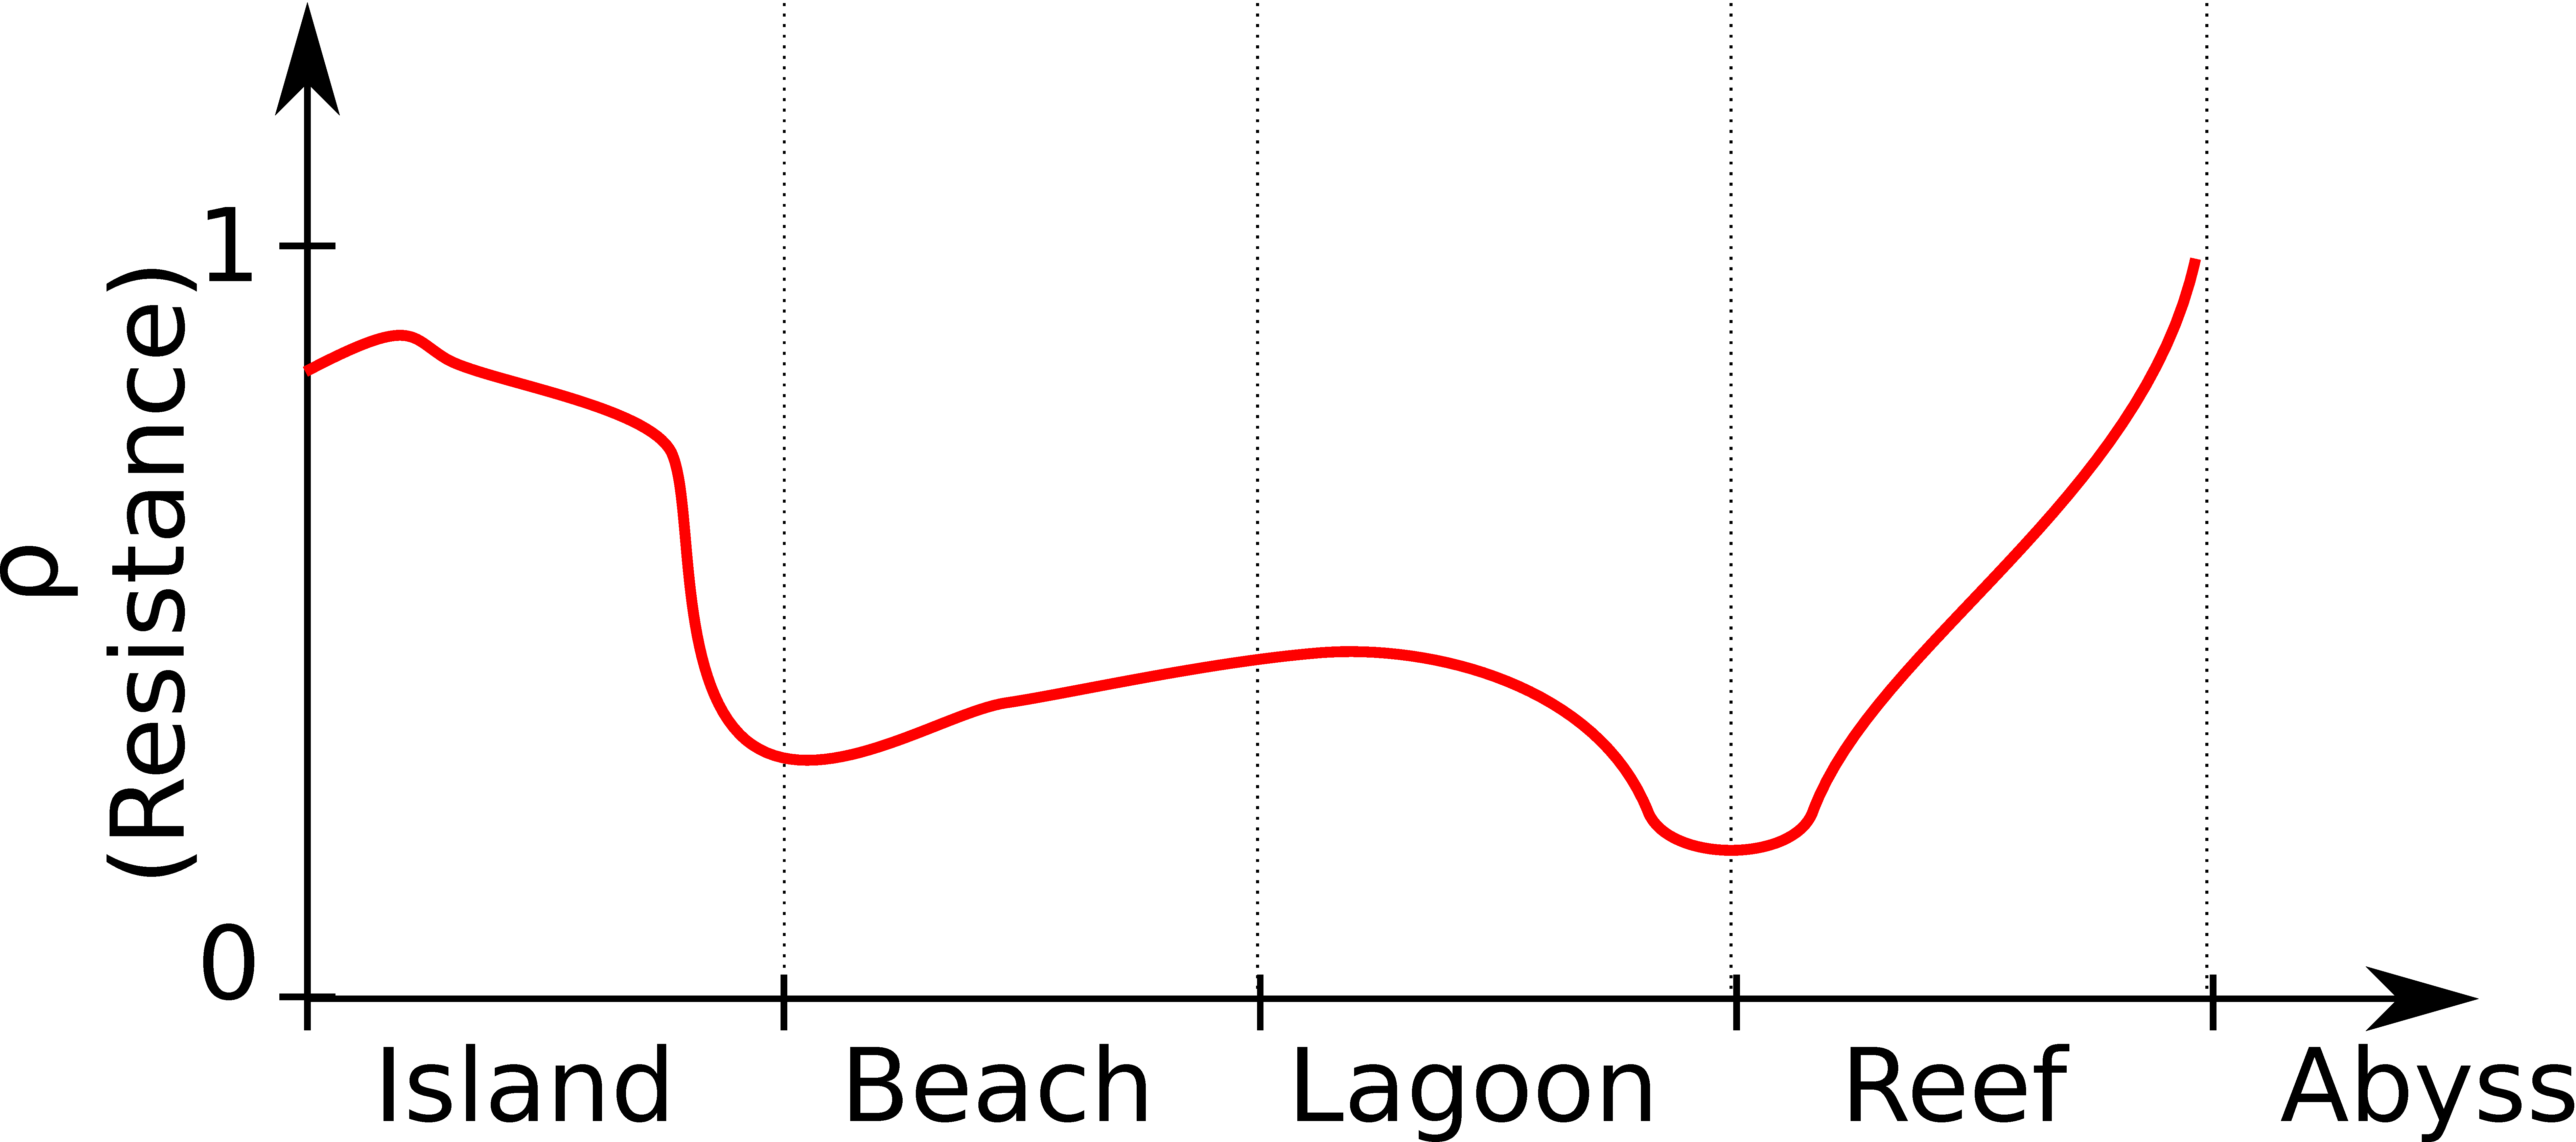
\includegraphics[width=0.45 \linewidth]{resistanceFunction.pdf}
%     \caption{The resistance function of the island is defined in the same way than the $\heightProfile$ function. The resistance to erosion and deformation arise from multiple factors such as depth, materials, wind shadowing, biotic and abiotic factors, ... Modeling all these factors is complex. As such, using a user-defined approximation through a resistance function $\resistance$ allows for more control. }
%     \label{fig:coral-island_resistance-function}
% \end{figure}



\subsection{Coral reef modeling}
\label{sec:coral-island_coral-reef}

Once the terrain has been generated and deformed by the wind, we simulate the long-term geological evolution of coral reef islands through two parallel processes: the subsidence of the volcanic island and the upward growth of coral reefs. As observed in nature, the volcanic base sinks over time while coral formations grow vertically to remain close to the water surface, following the "keep-up" strategy of reef development.

\subsubsection{Subsidence}
\label{sec:coral-island_subsidence}

Subsidence is modeled by uniformly scaling the original terrain height downward, simulating the gradual sinking of the volcanic landmass due to tectonic processes. The user specifies a subsidence rate $\subsidRate \in [0, 1]$, which controls how much the island has sunk. The subsided terrain is computed as:

\begin{align}
    \heightSubsid(\p) = (1 - \subsidRate) \cdot h_0(\p).
\end{align}

This factor is applied uniformly across the island, offering a geologically plausible and computationally efficient approximation of large-scale subsidence.

\subsubsection{Coral reef growth}
\label{sec:coral-island_reef-growth}

Coral reef growth is modeled independently from the subsiding terrain. The system generates a coral-specific height field $\heightCoral(\p)$ that remains near the sea surface regardless of the island's vertical shift, reflecting coral growth in biologically viable depth ranges (typically 0-30 meters below sea level).

\begin{figure}
    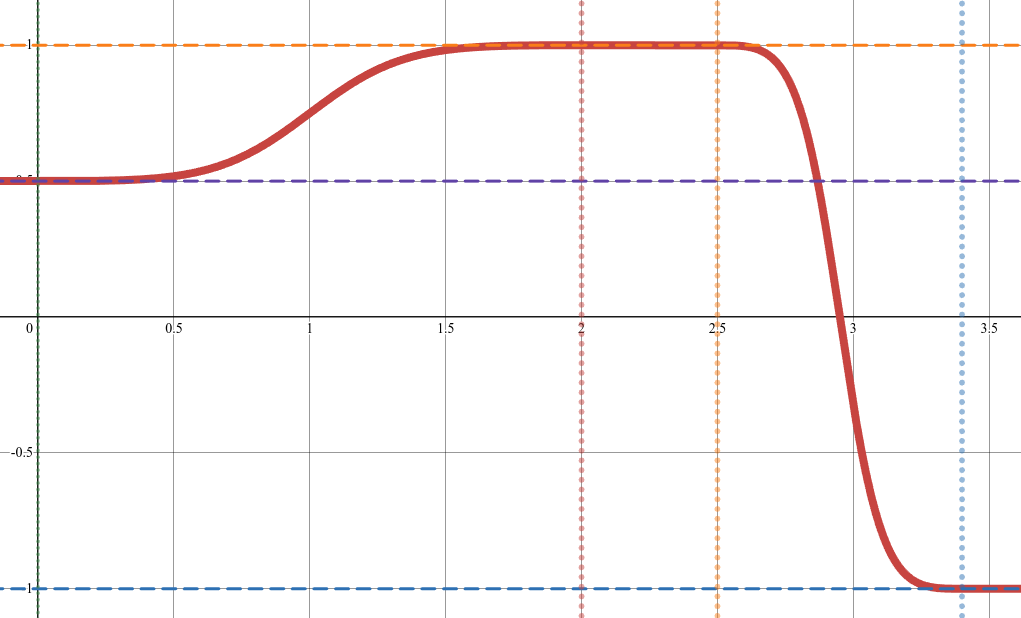
\includegraphics[width=0.7\linewidth]{Reef_function.png}
    \caption{The modeling of the reef growth in our model is described by a piecewise function $\heightCoral$ which is flat in the lagoon, the crest and abyss, and follows a smoothstep function as transitions for the backreef and fore reef regions. Zones' anchor heights are represented by horizontal dashed lines; zones' limits are dotted vertical lines. }
    \label{fig:coral-island_reef-function}
\end{figure}

We define distinct reef zones anchored at specific depths:
\begin{Itemize}
    \Item{} Reef crest near sea level: $h_\text{crest} = -2$\,m,
    \Item{} Back reef and lagoon: $h_\text{back} = -20$\,m,
    \Item{} Fore reef sloping to abyss: $h_\text{abyss} = -100$\,m.
\end{Itemize}

Each reef subregion is defined over a parametric domain $x \in [0, 1]$, with $x=0$ the begining of the reef region and $x=1$ its end, directly inputing the parametric distance $x = \distRegions - i_{\text{reef region}}$. For instance:
\begin{Itemize}
    \Item{} Back reef: $x_{\text{back,start}} = 0$, $x_{\text{back,end}} = 0.5$,
    \Item{} Reef crest: $x_{\text{crest,start}} = 0.75$, $x_{\text{crest,end}} = 0.8$,
    \Item{} Abyss begins at $x_{\text{abyss,start}} = 1$.
\end{Itemize}

We model transition zones between these regions using a smoothstep operator:
\begin{align}
    \smooth(x) = 3x^2 - 2x^3.
\end{align}

We denote the interpolating function as:
\begin{align}
    S(a, b, x_0, x_1, x) = a + (b-a) \smooth\left(\frac{x - x_0}{x_1 - x_0}\right).
\end{align}

The complete coral height field, as displayed in \cref{fig:coral-island_reef-function}, is built as a piecewise function:
\begin{align}
    \label{eq:coral-island_full-reef-function}
    &\heightCoral(x) = \sum_{r \in \text{subregions}}{
    \begin{dcases}
        h_r & \text{if } x_{\text{r,start}} \leq x \leq x_{\text{r,end}} \\
        0 & \text{otherwise}
    \end{dcases}
    } \nonumber \\ 
    &+
    \sum_{t \in \text{transitions}} {
        \begin{dcases}
            S(h_{t}, h_{t+1}, x_{\text{t,end}}, x_{\text{t+1,start}}, x) & \text{if } x_{\text{t,end}} < x < x_{\text{t+1,start}} \\
            0 & \text{otherwise}
        \end{dcases}
    }
\end{align}


% \subsubsection{Blending height fields}
% \label{subsubsec:height-functions-blending}

% \begin{figure}
%     \autofitgraphics[]{blend_function_low_approx.png, blend_function_high_approx.png}
%     \autofitgraphics[]{blend_compare_closeup_low.png, blend_compare_closeup_high.png}
%     \caption{Blending two functions $f: \R \to \R$ (black) and $g: \R \to \R$ (blue) with the $\max$ operator (red), causing a discontinuity, and with the $\smoothmax$ operator (green), resolving the issue at the cost of slight underestimations with low values of $k$. Left: $k=5$, right: $k=50$}
%     \label{fig:coral-island_blend-function-island}
% \end{figure}

% \begin{figure}
%     \autofitgraphics[]{blend_function_with_upper_low.png, blend_function_with_upper_high.png}
%     \autofitgraphics[]{blend_closeup_k_5.png, blend_closeup_k_10.png, blend_closeup_k_50.png}
%     \caption{The $\smoothmax^+$ operator(orange) is a function that use to overestimate the maximum value of two functions, especially when the difference between the two functions is small, while the $\smoothmax^-$ function (green) tends to underestimate the $\max$ operator. Taking $\smoothmax$ (red) as the average of $\smoothmax^-$ and $\smoothmax^+$ creates a much more precise blending, even with lower values of $k$ (Left: $k=5$, center: $k=10$, right: $k=50$).}
%     \label{fig:coral-island_blend-function-island-with-upper}
% \end{figure}

% The final step is to blend the subsided height field $\heightSubsid(\p)$ with the coral feature height field $\heightCoral(\p)$ to produce the final terrain. The goal is to ensure that coral features remain near the water surface while allowing the rest of the island to subside.

% To achieve this, the system uses a smooth max function, which smoothly blends the two height fields. The smooth max function ensures that the coral regions dominate where coral growth is present, while the subsided island terrain dominates in other regions. This blending method ensures that the transition between the coral and subsided regions is smooth and visually consistent.

% We define our smooth max function $\smoothmax: a, b \in \R^2$ as the mean of two functions, $\smoothmax^-$ and $\smoothmax^+$, adapted from Ingo Quilez's smooth min function, that respectively underestimate and overestimate the function $\max$:

% \begin{align}
%     \smoothmax^-(a, b) &= a + \frac{b - a}{1 + \exp\left(-k \cdot (b - a) \right)} \\
%     \smoothmax^+(a, b) &= a + \frac{b - a}{1 - \exp\left(-k \cdot (b - a) \right)} \\
%     \smoothmax(a, b)   &= a + \frac{\smoothmax^-(a, b) + \smoothmax^+(a, b)}{2} %}{2}
% \end{align}

% Here, $a = \heightSubsid(\p)$ is the height from the subsided island, $b = \heightCoral(\p)$ is the height from the coral reef feature, and $k$ controls the smoothness of the transition. Higher values of $k$ brings the $\smoothmax$ function closer to the $\max$ function (\cref{fig:coral-island_blend-function-island}).

% This smooth max function guarantees visual continuity by preventing abrupt height differences between the coral regions and the subsided terrain, creating a smooth, gradual transition that mimics the natural blending of coral reefs with deeper areas. The coral feature height field takes precedence where coral can grow, typically in shallow regions. In deeper regions, such as the abyss, the subsided height field naturally dominates, ensuring that the final terrain accurately reflects both subsidence and coral growth processes.

% Note that the $\smoothmax$ function is undefined for $a = b$, however, a proof of continuity for $\smoothmax \in C^\infty$ is provided in \cref{chap:smoothmax-proof} resulting in:
% \begin{align}
%     \smoothmax(a, b) = \begin{dcases}
%         a + \frac{1}{2k} & \text{ if } a = b, \\
%         \frac{\smoothmax^-(a, b) + \smoothmax^+(a, b)}{2} & \text{otherwise}
%     \end{dcases}    
% \end{align}

\subsubsection{Output}
\label{sec:coral-island_procedural-output}

\begin{figure}
    \autofitgraphics[]{volcano-input.png, volcano-render-corrected.png}
    \autofitgraphics[]{volcano-heightmap.png, volcano-corals.png, volcano-output.png}
    \autofitcaptions{Initial height field, Reef only, Blended height field}
    \caption{Volcano with single vent. (Bottom left) The initial height field is computed directly from the user input, (bottom center) the reef height field is outputed from \cref{eq:coral-island_full-reef-function}, and finally, (bottom right) we blend the two results with \cref{eq:coral-island_smoothmax-function}.}
    \label{fig:coral-island_volcano-example}
\end{figure}

Finally, we merge the island base height field and the coral reef height field by our \textit{ad-hoc} smooth maximum operator $\smoothmax$ defined as:
\begin{align}
    \label{eq:coral-island_smoothmax-function}
    \smoothmax(a, b) = \begin{dcases}
        % a + \frac{b - a}{2k} \left( \frac{1}{1+e^{-k(b - a)}} + \frac{1}{1-e^{-k(b-a)}} \right) &\text{for } a \neq b \\
        a + \frac{\delta}{2k} \left( \frac{1}{1+e^{-k\delta}} + \frac{1}{1-e^{-k\delta}} \right) &\text{for } a \neq b \\
        a + \frac{1}{2k} &\text{for } a = b
    \end{dcases}
\end{align} 
with $\delta=b-a$ for conciseness, and $k$ a sharpness parameter approximating the $\max$ operator as $k$ grows. At $k=5$, the operator $\max$ is already well approximated while conserving continuousness in the resulting height field $\height(p) = \smoothmax(\heightSubsid(\p), \heightCoral(\p))$.

The resulting terrain represents a plausible coral reef island, where the volcanic island has subsided, and coral reefs have grown upward to keep pace with the water level (\cref{fig:coral-island_volcano-example}). The smooth blending between the subsided terrain and the coral features ensures a natural transition between regions like the island, lagoon, and coral reefs.